\subsection{\label{s:laserMFnum}\Poincare\ section and slice combined}

In this section we demonstrate in the example of \cLe\
that we can reduce continuous symmetry and construct return maps
for high-dimensional flows even through a slice that is well
defined only locally, such as coordinate slice $x_1=0$
of \refsect{s:cleCoordSlice}.

Transformations \refeq{eq:invLaser} obtained
through use of {\mframes} with a coordinate \slice\
are singular in subspace $x_1=x_2=0$.
Therefore we would like to ensure that we apply our
reduction procedure only on points away from this subspace. A
way to achieve this is by a judicious choice of \Poincare\
section in original space, \ie~before reduction. Since we are
ultimately interested in reducing the dynamics to a
\Poincare\ return map this suffices for our purposes.
Different \Poincare\ sections that intersect the same orbits provide conjugate return
maps with essentially the same information. This allows great freedom to avoid
group-action-induced singularities.
Locating a \Poincare\ section is a non-trivial task
but as we will see in the following, for the procedure to
work we will have to reduce the candidate \Poincare\ sections
to those that are invariant (as a set) under the group
action. Here we are naturally led to choose a section that passes through
\reqv~\REQV{}{1} such as section \PoincS\
defined by $\overline{x}_2-\overline{y}_2=0$ in the variables
of \refeq{eq:invLaser} or by $x_1^2+x_2^2-(x_1 y_1 + x_2
y_2)=0$ in original space and a suitable orientation
condition so that trajectories intersect the section away
from $x_1=x_2=0$ subspace. Here the orientation condition has
be chosen so that trajectories intersect \PoincS\ moving
from the ``outside'' of the section in
\reffig{fig:CLEmartini} to the ``inside.'' Since
\PoincS\ has been defined by a condition in invariant
variables \refeq{eq:invLaser} it is
$\SOn{2}$-invariant in equivariant variables. Therefore the group
orbit of any point on \PoincS\ lies on \PoincS. In
\reffig{fig:CLEmartini} the group orbits of points of
intersection of \rpo~\cycle{01} are visualized as circles
on \PoincS.

The next step is to choose a representative out of each group
orbit by means of a \slice\ that intersects each group orbit
exactly once. Since Poincar\'e section \PoincS\ has been
chosen to lie away from $x_1=x_2=0$, even a simple coordinate
slice, such as $\pSRed$ defined by $x_1=0$ is adequate.
Geometrically this is equivalent to rotating each point of
intersection on ${\pSRed}$ by an appropriate angle so that it
lies on $\pSRed$, exactly as prescribed by
\refeq{cLeCoordTheta}. As we remarked in \refsect{s:mfReqb}
this rotation, a linear operation for any given point, can be
applied efficiently even in a high dimensional
space.
    \ES{Restore and refer to return map of coordinate slice
section.}

%%%%%%%%%%%%%%%%%%%%%%%%%%%%%%%%%%%%%%%%%%%%%%%%%%%%%%%%%%%%%%%%%%
\begin{figure}[ht]
\begin{center}
  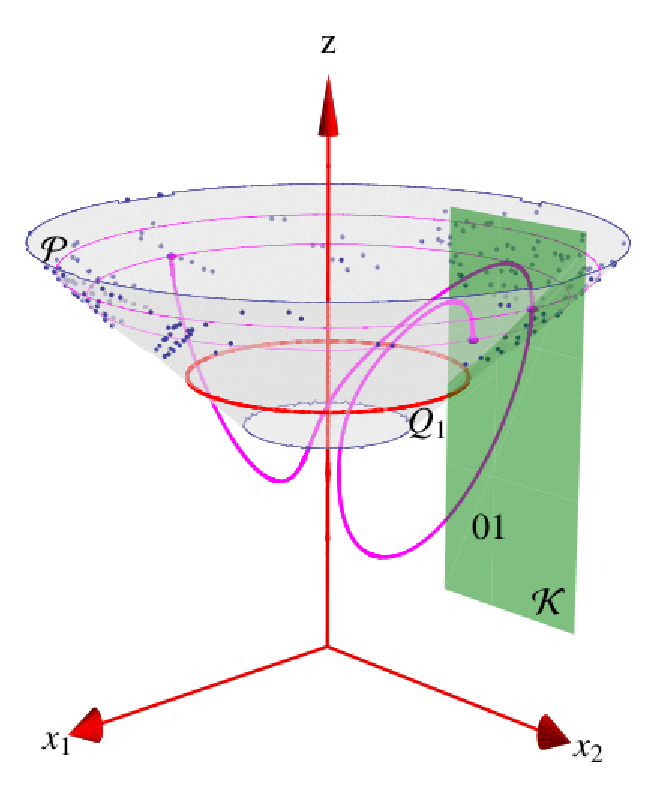
\includegraphics[width=0.35\textwidth]{CLEmartini}
\end{center}
\caption{
Use of \Poincare\ surface of section \PoincS\ and
{\slice} $\pSRed$ for symmetry reduction of \cLe\
dynamics. Group orbits of the points of intersection of \rpo\
\cycle{01} are visualized as circles.
    }
\label{fig:CLEmartini}
\end{figure}
%%%%%%%%%%%%%%%%%%%%%%%%%%%%%%%%%%%%%%%%%%%%%%%%%%%%%%%%%%%%%%%%
